\documentclass{article}
\usepackage{graphicx} % Required for inserting images
\usepackage{amsmath}


\title{Assignment 2}
\author{Steven Sanchez}
\date{January 2026}


\begin{document}

\maketitle


\section*{Question 1}
\subsection*{Part (a):}
\begin{center}
$\hat{y}^{(i)} = sign(w \cdot x^{(i)})$, 

sign$(z) = (1, z>=0)$ or $(-1, z < 0)$


$(y^{(i)} \in {-1, 1})$


$w = w + y^{(i)}x^{(i)}$
\end{center}

\begin{center}
\begin{tabular}{|c|c|c|c|}
\hline
$i$ & $x_1^{(i)}$ & $x_2^{(i)}$ & $y^{(i)}$ \\
\hline
1 & 1 & 1 & 1 \\
2 & 2 & -1 & -1 \\
3 & -3 & -1 & 1 \\
4 & -3 & 1 & 1 \\
\hline
\end{tabular}
\end{center}

starting with $w$ = [0 0]$^{T}$, we will use the perceptron algorithm to learn on the data points in order $i = 1, 2, 3, 4$.
\begin{center}
$x^{(1)} = (1, 1)$, $y^{(1)} = 1$

$x^{(2)} = (2, -1)$, $y^{(2)} = -1$

$x^{(3)} = (-3, -1)$, $y^{(3)} = 1$

$x^{(4)} = (-3, 1)$, $y^{(4)} = 1$
\end{center}
i = 1, w = (0, 0), z = (0,0) * (1, 1) = 0,
$\hat{y}^{(i)} = sign(0) = 1$


-

i = 2, w = (0, 0), z = (0, 0) * (2, -1) = 0, 
$\hat{y}^{(i)} = sign(0) = 1$
In this one, our actual y label is -1, but we predicted 1, so this is wrong here. With this, we 
will update our w to $w = (0, 0) + (-1)(2, -1) = (-2, 1)$

-

i = 3, w = (-2, 1), z = (-2, 1) * (-3, -1) = (-2)(-3) + (1)(-1) = 6 - 1 = 5
,

sign(5) = 1, this is correct so we keep our w the same.

-

i = 4, w = (-2, 1), z = (-2, 1) * (-3, 1) = (-2)(-3) + (1)(1) = 6 + 1 = 7, sign(7) = 1, and this one is also correct.

-

Our final $w = (-2, 1)$. 

-

i = 1, w = (-2, 1), z = (-2, 1) * (1, 1) = (-2)(1) + (1)(1) = -2 + 1 = -1, sign(-1) = 0 , which is wrong since our y here is 1.

-

i = 2, w = (-2, 1), z = (-2, 1) * (2, -1) = (-2)(2) + (1)(-1) = -4 - 1 = -5, sign(-5) = -1 which is correct

-

i = 3, w = (-2, 1), z = (-2, 1) * (-3, -1) = (-2)(-3) + (1)(-1) = 6 - 1 = 5, sign(5) = 1, which is correct

-

i = 4, w = (-2, 1), z = (-2, 1) * (-3, 1) = (-2)(-3) + (1)(1) = 6 + 1 = 7, sign(7) = 1 which is correct

-

In conclusion, our final w predicted 3/4 of them, with our first i = 1 being predicted wrong. 

\subsection*{Part (b):}

i = 2, w = (0, 0), z = (0, 0) * (2, -1) = (0)(2) + (0)(-1) = 0, sign(0) = 1, which is wrong since the real y = -1, so we will update our w. 


w = (0,0) + (-1)(2, -1) = (-2, 1)

-

i = 1, w = (-2, 1), z = (-2, 1) * (1, 1) = (-2)(1) + (1)(1) = -2 + 1 = -1, sign(-1) = -1, which is wrong again since our true y = 1. so we will update our w again

w = (-2, 1) + (1)(1, 1) = (-2 + 1, 1 + 1) = (-1, 2)

-

i = 3, w = (-1, 2), z = (-1, 2) * (-3, -1) = (-1)(-3) + (2)(-1) = 3 + 1 = 4, sign(4) = 1, so this is correct

i = 4, w = (-1, 2), z = (-1, 2) * (-3, 1) = (-1)(-3) + (2)(1) = 3 + 2 = 5, sign(5) = 1, so this is correct


Our final $w = (-1, 2)$, now to check if it correctly classifies all data points:


i = 1, w = (-1, 2), z = (-1, 2) * (1, 1) = (-1)(1) + (2)(1) = -1 + 2 = 1, sign(1) = 1 which is correct

-

i = 2, w = (-1, 2), z = (-1, 2) * (2, -1) = (-1)(2) + (2)(-1) = -2 - 2 = -4, sign(-4) = -1 which is correct

-

i = 3, w = (-1, 2), z = (-1, 2) * (-3, -1) = (-1)(-3) + (2)(-1) = 3 - 2 = 1, sign(1) = 1 which is correct

-

i = 4, w = (-1, 2), z = (-1, 2) * (-3, 1) = (-1)(-3) + (2)(1) = 3 + 2 = 5, sign(5) = 1 which is correct


In conclusion, this order does compute all data points correctly, is this order got 4/4 correct.
$w = (-1, 2)$


\section*{Question 2}

Data point: $x = [x_1, x_2] \in R^2$

Hidden layer: $z = w \cdot x$ where $z \in R$ and the weight vector $w = [w_1, w_2] \in R^2$

Output layer: produces a prediction $\hat{y}$ = sigmoid($z$)

Use error $(\hat{y} - y)^2$ to measure prediction loss where $y$ is the true label

input $x = [1, 0]$, true label $y = 1$, initial weight vector $w = [-1, 2]$

-

$x = [1, 0]$, true label: $y = 1$, initial weight vector: $w = [-1, 2]$

-

loss = $(\hat{y} - y)^2$

-

$\hat{y} = sigmoid(z) = \frac{1}{1+e^{(-z)}}$

-

z = w * x = (-1, 2) * (1, 0) = (-1)(1) + (2)(0) = -1, so z = -1

then, sigmoid(z) = sigmoid(-1) = $\frac{1}{1+e^1}$ = 0.2689

\begin{figure}[h]
    \centering
    
\includegraphics[width=0.4\linewidth]{image1.png}
    \label{fig:placeholder}
\end{figure}

loss: $(\hat{y} - y)^2 = (0.2689 - 1)^2 = 0.5344$

\begin{figure}[h]
    \centering
    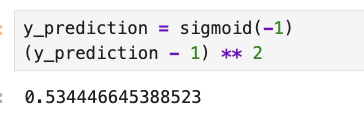
\includegraphics[width=0.4\linewidth]{image2.png}
    \label{fig:placeholder}
\end{figure}

Now for the backward pass: 

$\frac{\partial loss}{\partial w_1}$ and $\frac{\partial loss}{\partial w_2}$, 

Loss = $(\hat{y} - y)^2$, where the derivative is $2(\hat{y} - y)$, so we will compute that by plugging in our numbers.

$\frac{\partial Loss}{\partial \hat{y}} = 2(\hat{y} - y) = 2(0.2689 - 1) = -1.462$
\begin{figure}[h]
    \centering
    
\includegraphics[width=0.4\linewidth]{image3.png}
    \label{fig:placeholder}
\end{figure}

,

\begin{figure}[h!]
    \centering
    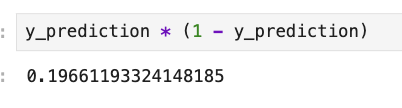
\includegraphics[width=0.4\linewidth]{image4.png}
    \label{fig:placeholder}
\end{figure}

now for the sigmoid function, $\frac{\partial Loss}{\partial z}$ = $\hat{y}(1 - \hat{y}) = 0.2689(1 - 0.2689) = 0.1966$, with the image above since latex wouldn't let me put it directly below this text.

$\frac{\partial z}{\partial w_1} = x_1 = 1$


$\frac{\partial z}{\partial w_2} = x_2 = 0$


$\frac{\partial Loss}{\partial w_1} = (-1.462) \cdot (0.1966) \cdot 1 = -0.287$

\begin{figure}[h]
    \centering
    
\includegraphics[width=0.5\linewidth]{image5.png}
    \label{fig:placeholder}
\end{figure}


$\frac{\partial Loss}{\partial w_2} = (-1.462) \cdot (0.1966) \cdot 0 = 0$

\begin{figure}[h]
    \centering
    
\includegraphics[width=0.5\linewidth]{image6.png}
    \label{fig:placeholder}
\end{figure}

$(w_1)$ -

----------- $\cdot$ $(z_1)$

$(x_1)$ -

,

-------------------- $=(z_i)$ --- $(sigmoid(z))$ --- $(\hat{y} - y)$ --- $(\hat{y} - y)^2$ --- $Loss$

,

$(w_2)$ -

----------- $\cdot$ $(z_2)$

$(x_2)$ -


\section*{Question 3}

single neuron with scalar input $x \in R$, scalar weight $w$, and bias $b$

-

$z = wx + b$, $\hat{y} = \phi (z)$,

with squared error loss:

$L = \frac{1}{2}(\hat{y} - y)^2$

-

We use the ReLU activation: $\phi (z) = max(0, z)$.

\subsection*{Part (a):}

\begin{center}
$\frac{\partial \phi (z)}{\partial z}$
\end{center}

I found this piecewise online as I didn't know how to add the symbol on latex, so I imported the module needed at the beginning of the latex file.

\begin{equation}
\phi(z) = max(0, z) = 
\begin{cases}
0 & \text{if } z  \le 0 \\
z & \text{if } z > 0
\end{cases}
\end{equation}

Therefore, taking the derivative would give us:

\begin{equation}
\frac{\partial \phi (z)}{\partial z} = 
\begin{cases}
0 & \text{if } z  \le 0 \\
1 & \text{if } z > 0
\end{cases}
\end{equation}

\subsection*{Part (b):}

\begin{center}
derive $\frac{\partial L}{\partial w}$ in terms of $x$, $y$, and $z$.
\end{center}

$L = \frac{1}{2}(\hat{y} - y)^2$, so the derivative is$\frac{\partial L}{\partial y}$ = $(\hat{y} - y)$, where you bring the squared number down (2) and multiply that by ($\frac{1}{2}$), which practically cancel each other out. 

$\hat{y} = \phi(z)$, $\frac{\partial \hat{y}}{\partial z}$ = $\phi ' (z)$ where $z = w \cdot x$, so $\frac{\partial z}{\partial w} = x$

Combining these terms, we get:

$\frac{\partial L}{\partial w} = \frac{\partial L}{\partial \hat{y}} \cdot  \frac{\partial \hat{y}}{\partial z} \cdot \frac{\partial z}{\partial w}$ = $(\hat{y} - y) \cdot \phi '(z) \cdot x$

\subsection*{Part (c):}

Finding all conditions on $x, w, b,$ and $y$ under which $\frac{\partial L}{\partial w}$ = 0, but $\hat{y} \ne y$.

$\frac{\partial L}{\partial w} = (\hat{y} - y) \cdot \phi '(z) \cdot x$
For this to be zero, at least $\phi(z)$ or $x$ must be zero since our $(\hat{y} - y)$ can't be zero. So with the ReLU activation, if $z < 0$, then the gradient is still zero since:

$\hat{y} \ne y$, $\hat{y} = \phi(z) = 0$ so our gradient would be zero.

If our $\hat{y} = 0$ and $\hat{y} \ne y$, then that means that z < 0, or equivalently, $wx + b < 0$.

To conclude, $\frac{\partial L}{\partial w} = 0$ when $x = 0$ and when $\phi(z) = 0$. 

\subsection*{Part (d):}

The reason why the gradient descent will not update w even though the neuron is making an error is because the model will get to a point where the gradient is zero. When this happens, when the model tries updating the weight, the gradient is multiplied by the derivative of the ReLU activation, which will be zero. Since this will happen, the gradient descent will have no way of knowing to change the weight and will be stuck. 

\subsection*{Part (e):}

The leaky ReLU activation is:

\begin{equation}
\phi(z) = 
\begin{cases}
\alpha z & \text{if } z  < 0 \\
z & \text{if } z \ge 0
\end{cases}
\end{equation}

for some small $\alpha> $ 0.

Just be looking at the piecewise equation above, we can see that if we take the derivative of $\alpha z$, our answer would actually be $\alpha$, rather than 0. Because of this, our gradient would look like:

$\frac{\partial L}{\partial w} = (\hat{y} - y) \cdot \phi '(z) \cdot x$  ---$>$
\begin{equation}
\phi('z) = 
\begin{cases}
\alpha & \text{if } z  < 0 \\
1 & \text{if } z \ge 0
\end{cases}
\end{equation}
---$>$ $\frac{\partial L}{\partial w} = (\hat{y} - y) \cdot \alpha \cdot x$, 



meaning that because the gradient is a non zero, even when our $z < 0$, our weight will continue to update. This means that our gradient descent can keep updating w and push us up to a positive range. 





\end{document}

